\chapter{Background\label{cha:background}}
This chapter describes the technologies and terminologies that are most important for the proposed solution, and puts them into context.

In \ref{sec:cloud-systems} a description of the term cloud computing is given. In \ref{sec:deep-learning} the theoretical foundation of deep neural networks is described, followed by an introduction to LSTMs. \ref{sec:natural-language-processing} gives insights on how natural language can be represented using language models.
In \ref{sec:anomaly-detection} techniques on tackling the problem of anomaly detection with deep learning techniques are presented.

\section{Cloud Computing\label{sec:cloud-systems}}
The term \textit{cloud computing} usually refers to hardware and systems software in large data centres that provide a platform for applications delivered as services over the Internet. Due to the possibilities offered by clouds that are available in a pay-as-you-go manner, businesses with new ideas do not require enormous amounts of prefinancing in a hardly projectable amount of hardware and human operators to get their services online. It allows them to dynamically adapt to changing business needs without neither overcommitting hardware for services that do not turn out to be as intensely used as expected, nor undercommitting for a service that excels expectations, thus missing potential revenue, due to not being able to cope with the demand \cite{armbrust2010view}.

Virtualisation plays a vital role in modern clouds, offering the possibility for numerous users and their applications to share infrastructure in parallel, in contrast to conventional hosting, as depicted in figure \ref{fig:virtualisation}. Through virtualisation, it is possible to achieve a better degree of utilisation of available hardware, for it allows a hardware server to run multiple software servers at the same time. Modern cloud services providers, like Amazon AWS or Microsoft Azure offer a vast number of different useful services, that can be provisioned flexibly and rapidly to the user, like allocation of task-specific hardware, different database types, object storage solutions or applications like analysis or management tools, as depicted in figure \ref{fig:cloud}. End customers can be individual persons or businesses. While the services offered by public cloud providers are usually full-fledged and can be used by an end customer directly, the services offered by a cloud provider can also be integrated into a private cloud solution, thus resulting in a hybrid cloud, where workloads can be dynamically shifted between private and public clouds as costs and computing capacity needs change.


Making sure that these large numbers of services and virtual machines are operating correctly is a challenging task for the cloud service providers. It is therefore vital to keep records of program executions in the form of logs to be able to retrace errors that have occurred.

\begin{figure}[h]
  \centering
  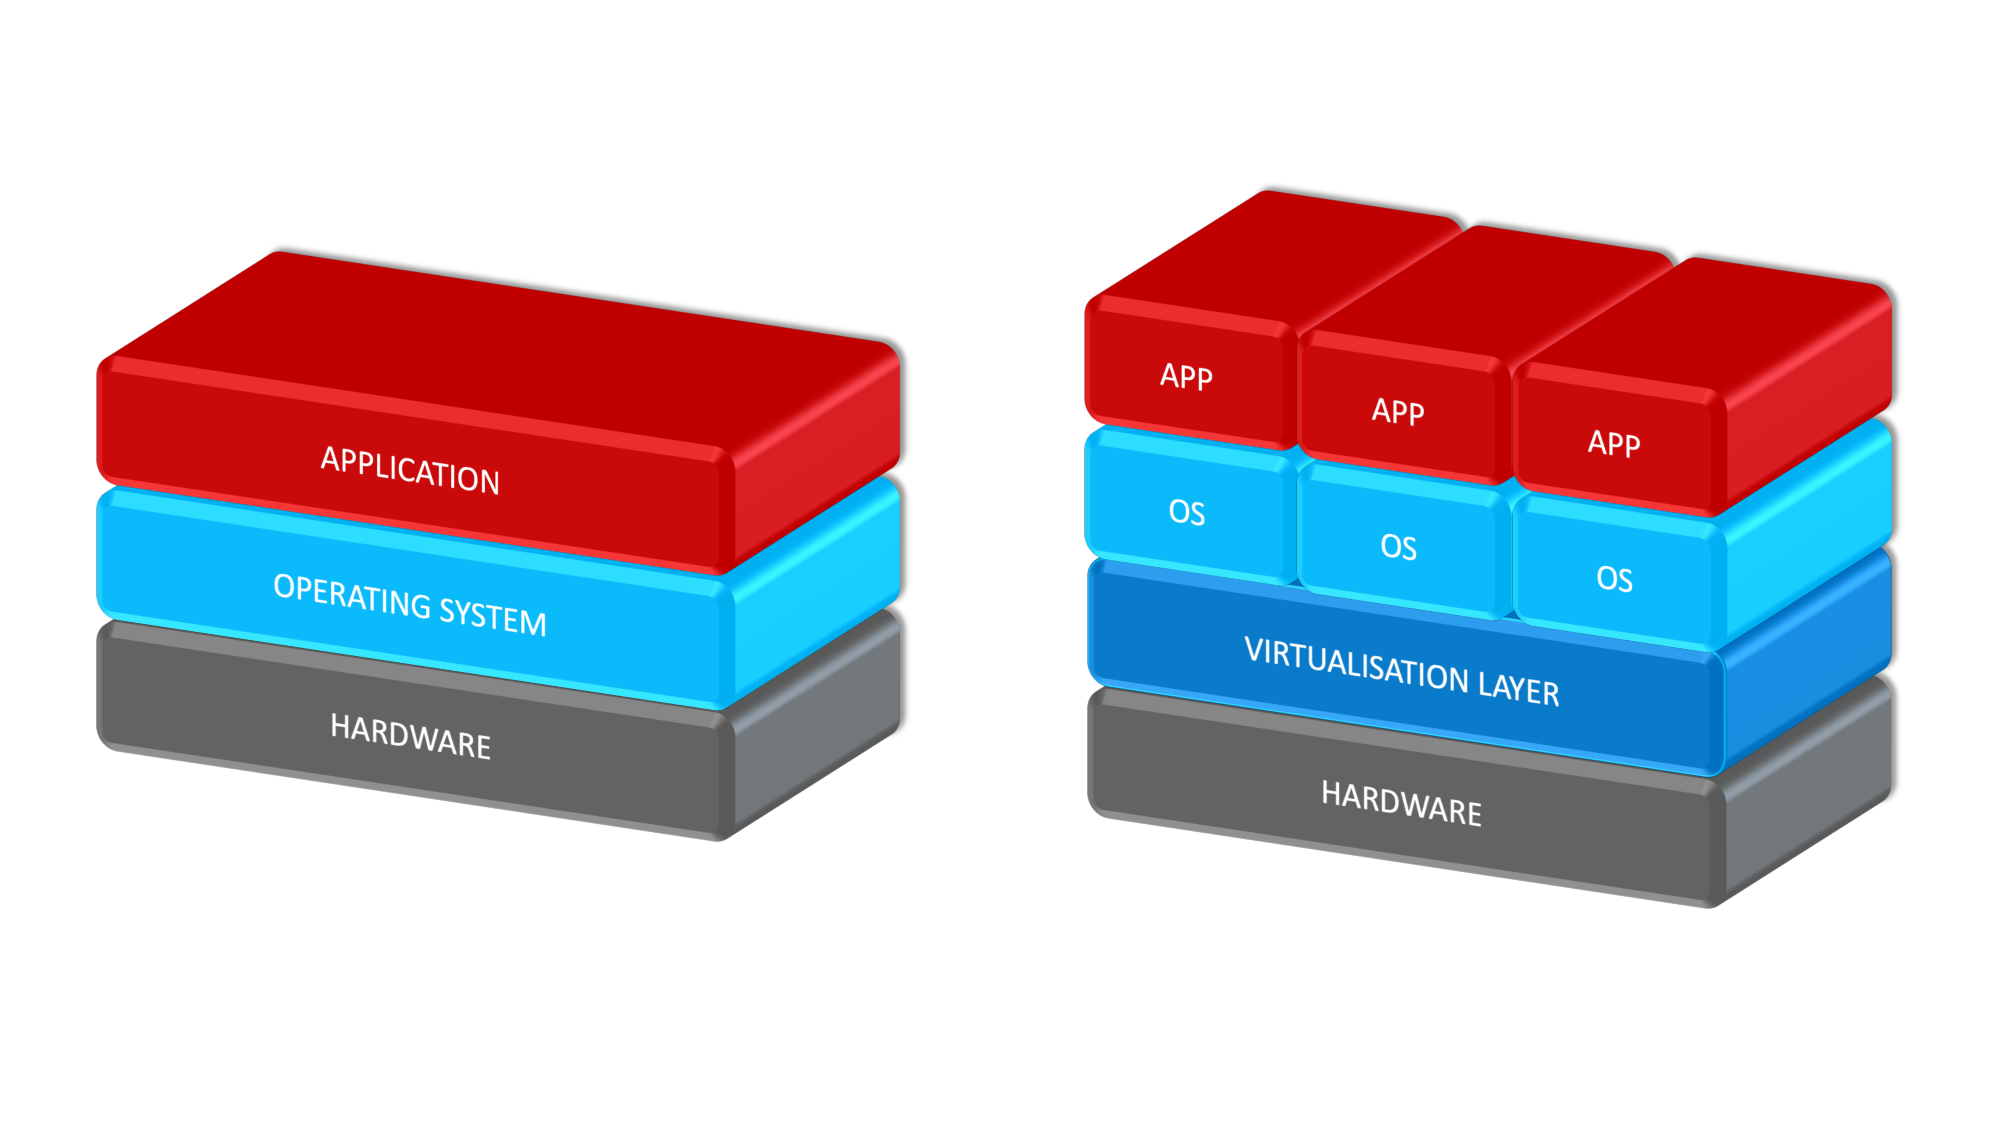
\includegraphics[width=10cm]{from_normal_to_virtualisation.pdf}\\
  \caption{Traditional architeture vs. virtualised architecture}
  \label{fig:virtualisation}
\end{figure}

\begin{figure}[h]
  \centering
  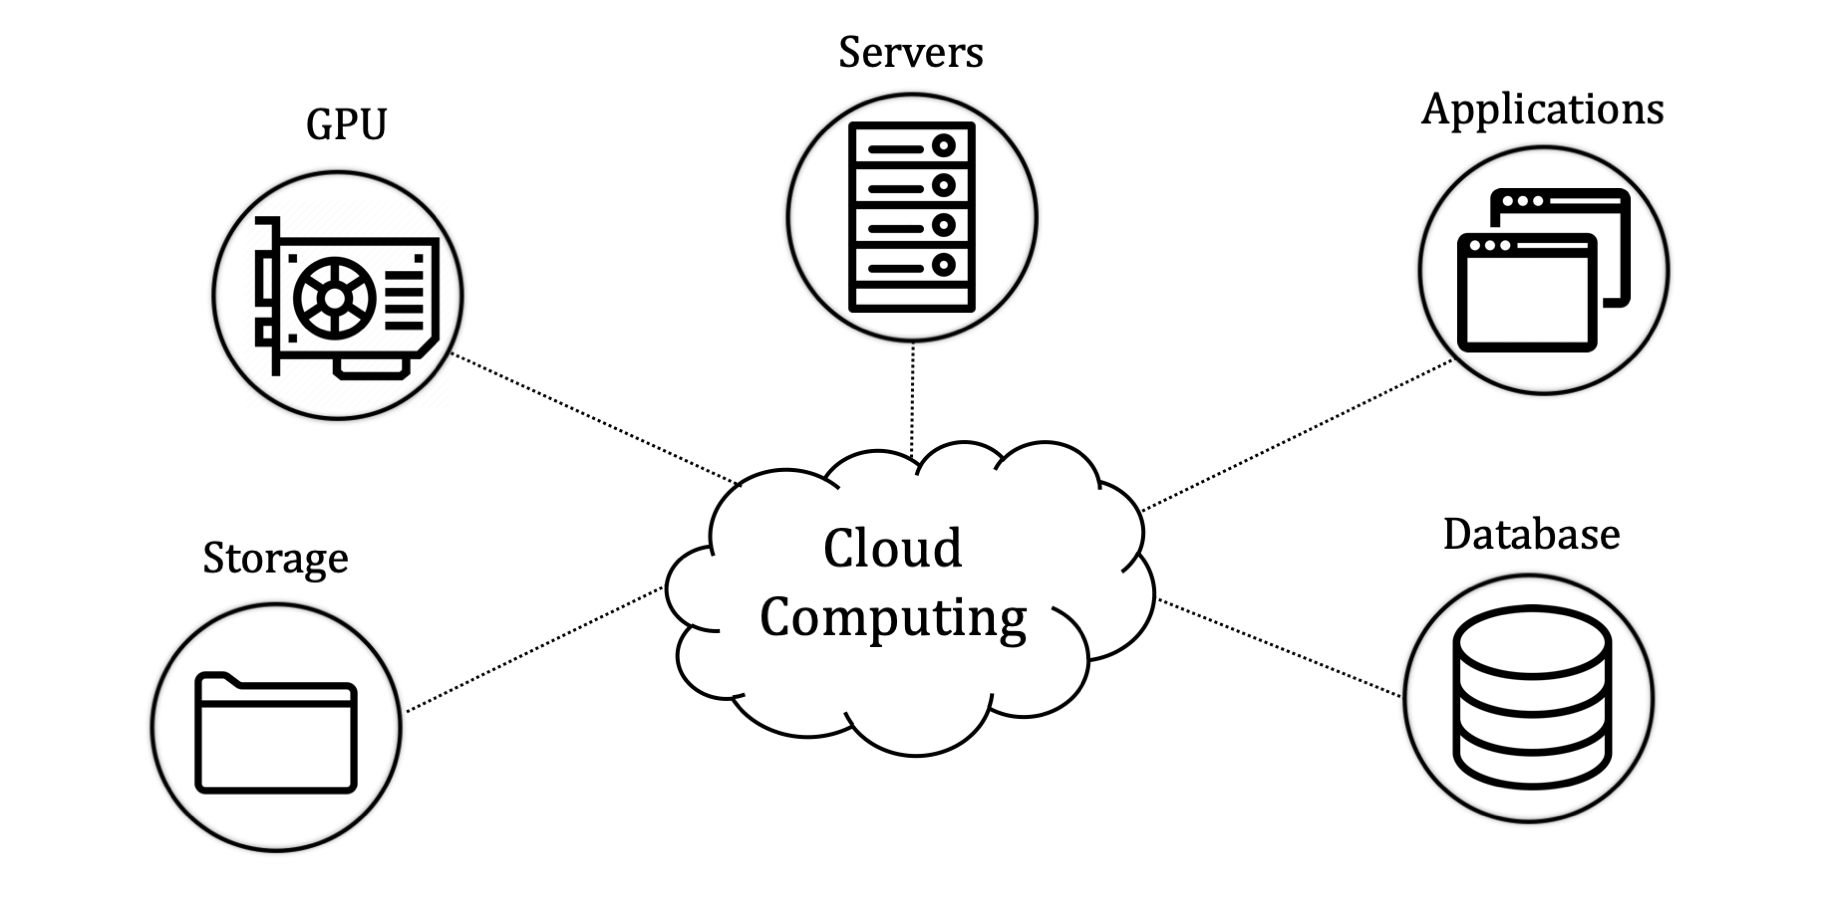
\includegraphics[width=15cm]{cloud.png}\\
  \caption{Traditional architeture vs. virtualised architecture}
  \label{fig:cloud}
\end{figure}


\section{Deep Learning \label{sec:deep-learning}}
\subsection{Neural Networks \label{sec:neural-networks}}
\begin{figure}[h]
  \centering
  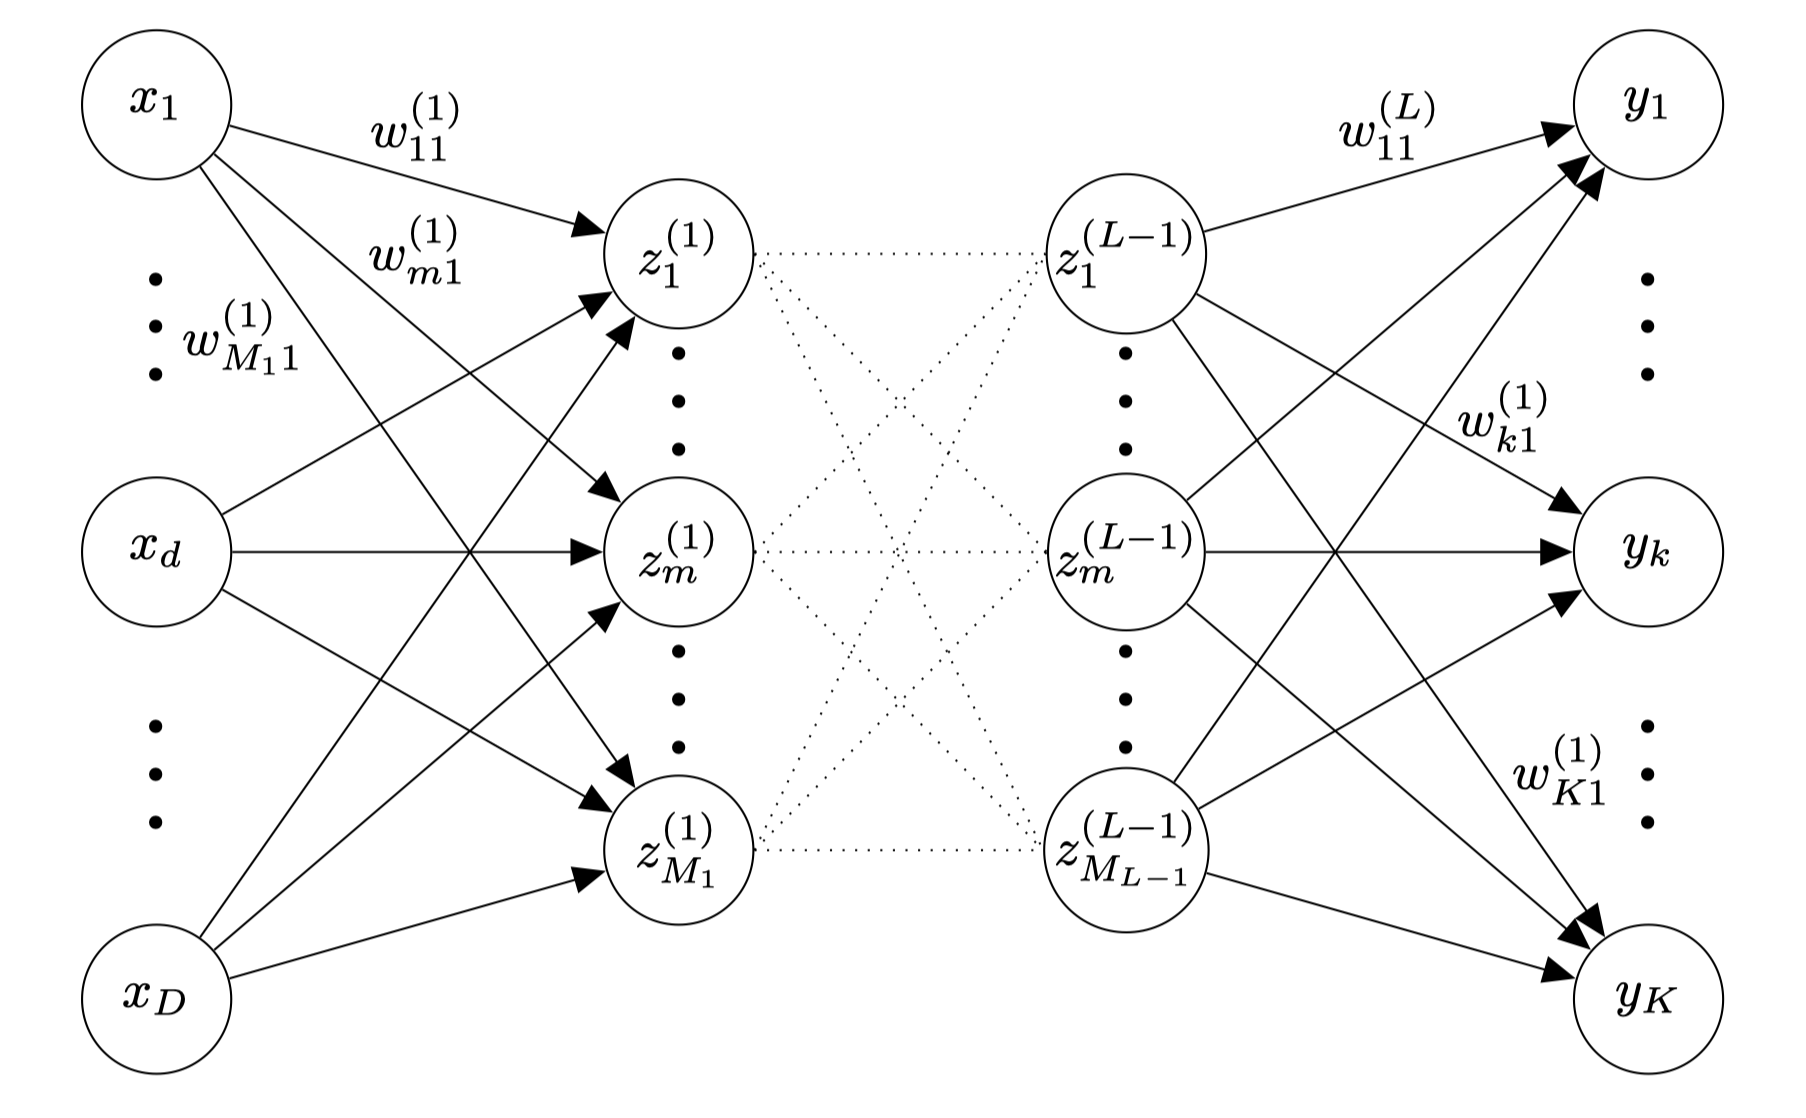
\includegraphics[width=15cm]{neural_network.png}\\
  \caption{A neural network \cite{hallmachinelearning}.}
  \label{fig:neural_network}
\end{figure}
Neural networks are self-learning systems that constitute a subcategory of machine learning. By analysing training examples, it learns to compute a functional relationship between an input and an output \cite{sibi2013analysis}. Figure \ref{fig:neural_network} is an illustration of a classical feed-forward neural network. It consist of \textit{neurons} and \textit{weights} connecting the neurons. There are three types of neurons: Each input value maps to an \textit{input} neuron depicted as $x_n$. \textit{Hidden} neurons, depicted as $z_i$ are predictors created by mathematical functions and the \textit{output} neurons, depicted as $y_k$ gather given predictions and compute the output \cite{hallmachinelearning}. Given data pairs $(x_1, t_1), ..., (x_N, t_N)$ with $x_n \in \mathbb{R}^D$ being input data, mapping to $D$ input neurons, and $t_n \in \mathbb{R}^K$ being target data. Each component $x_n$ is fed to one input neuron. If $L$ is the number of layers, then there are $L-1$ hidden layers. The network's latent variables of the hidden neurons are denoted by $z_m^{(l)}$. When data is being forwarded through the network, with the goal of obtaining a prediction from the network, the following formulas are relevant and describe every step through the network. The result of a complete forward propagation is denoted by activation \ref{eq:activation}:

\begin{equation}\label{eq:activation}
	a_j^{(l)} = \sum_{i=1}^{M_{l-1}}w_{ji}^{(l)}z_i^{(l-1)} = \bold{w}_j^{(l)^T} \bold{z}^{(l-1)}	
\end{equation}

On the result of this computation, an \textit{activation function} is applied as in \ref{eq:zj}. There exists a variety of activation functions, depending on the use case. Activation functions transform the activation of output neurons as in \ref{eq:activation} into an output signal \cite{sibi2013analysis}. For \textbf{regression} problems, the linear activation function $h(x)=x$ can be used. For \textbf{multi-classification} problems, where $t_n$ is a set of classes, the softmax function $\sigma(a)_j= \frac{e^{a_j}}{\sum_{k=1}^Ke^{a_k}}$ is used \cite{hallmachinelearning}.

There are more cases, but regression and multi-classification are the most relevant here, as they are used in chapter \ref{cha:concept}.

\begin{equation} \label{eq:zj}
	z_j^{(l)} = h_l(a_j^{(l)}) = h_l\Big(\bold{w}_j^{(l)^T} \bold{z}^{(l-1)}\Big)	
\end{equation}
If $l=1$, then equations \ref{eq:aj1} and \ref{eq:zj1} hold:

\begin{equation} \label{eq:aj1}
	a_j^{(1)}=\bold{w}_j^{(1)^T}\bold{x}
\end{equation}

\begin{equation} \label{eq:zj1}
	z_j^{(1)}=h_1\Big(\bold{w}_j^{(1)^T}\bold{x}\Big)
\end{equation}
If $l=L$, then every $y_k$ can be obtained in the following way:

\begin{equation}
	y_k = h_L(a_k^{(L)}) = h_L\Big( \bold{w}_k^{(L)^T} \bold{z}^{(L-1)} \Big)
\end{equation}

The result $y_k$ of the computation of $x_k$ is then compared to the real value $t_k$ using an \textit{error function}. Mean Squared Error $MSE = \frac{1}{n} \sum_{i=1}^n (t_k-y_k)^2$ can be used for regression problems, calculating the average squared difference between the estimated and the actual values, and Cross-Entropy $-\sum_{c=1}^My_{o,c} \: \log(p_{o,c})$ for multiclass classification, calculating the separate loss for each class label per observation. The obtained values are then fed into the \textit{back propagation algorithm}, updating weights $w_j$, thus trying to minimise the error. 


\begin{comment}
Figure \ref{fig:simple_neural_network} shows a simple neural network with three input features $v_1, v_2, v_3$. The output neuron is composed of the forward propagation function given by the weighted sums of neuron values, where the weights are $w_i$, and the activation function given by $h$. There exists a large variety of activation functions in use, depending on the given use case. The learning process of a neural network consists of learning the weights

Training of a neural network happens through 
Training of a neural network can be done in an \textit{unsupervised} and \textit{supervised} manner. Supervised training of 
The complexity of neural networks can be increased by adding more neurons and additional layers, making it possible to process larger input and potentially receive better results in prediction. The concept of the traditional feedforward neural networks is subject to constant architectural enhancement. 

Through the surge of available cheap computing power, deep learning models with high numbers of layers of neurons can be trained on large amounts of data. Also, the concept of the traditional neural network is constantly being 
\end{comment}



\subsection{LSTM networks \label{sec:lstm}}
\begin{figure}[h]
  \centering
  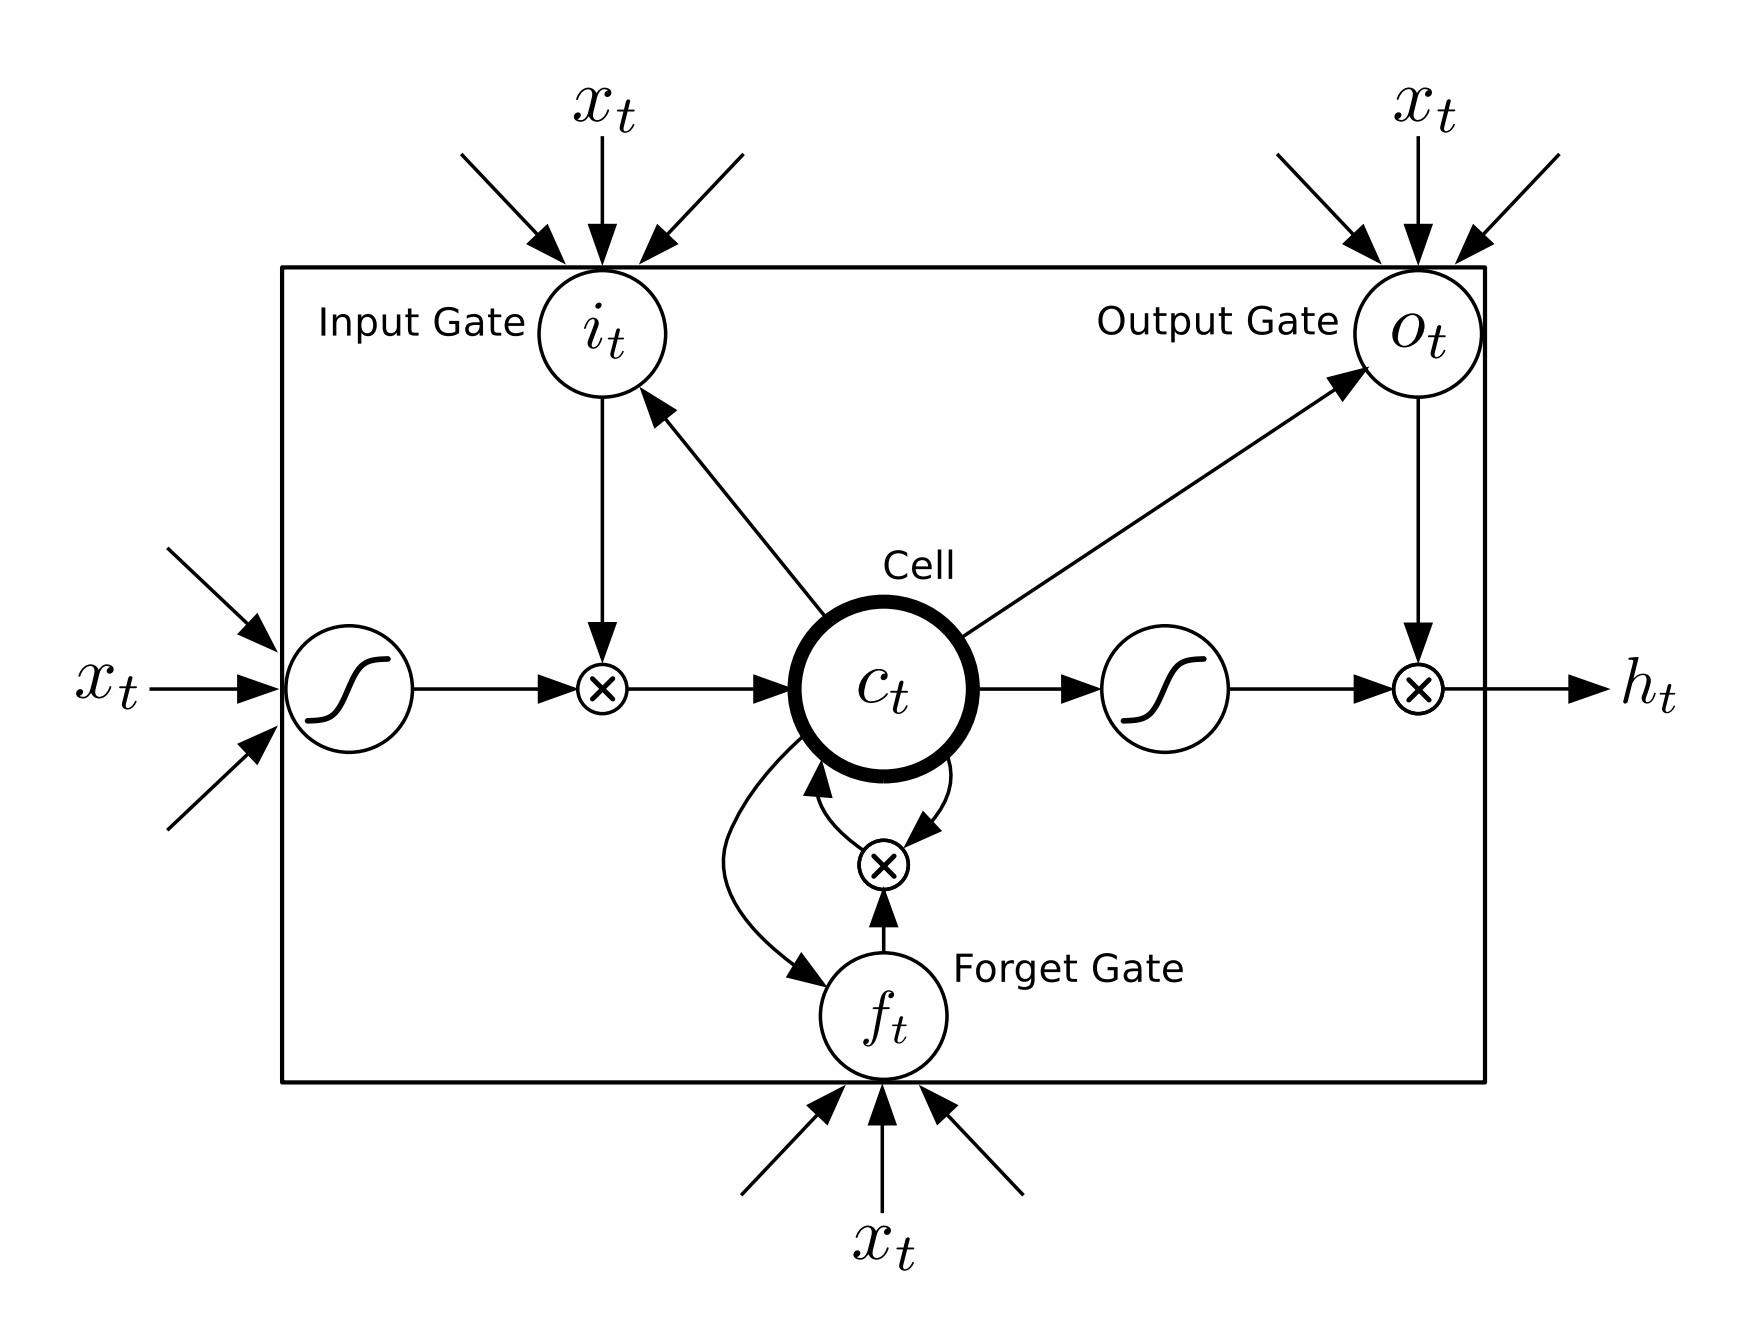
\includegraphics[width=10cm]{LSTM.png}\\
  \caption{LSTM block \cite{graves2013speech}}
  \label{fig:lstm_blocks}
\end{figure}


Recurrent neural networks (RNN) with Long Short-Term Memory (LSTM) are a widely-used effective model to tackle learning problems on sequential data. Being a general model, they do not have be to be adapted to a specific problem like earlier methods, thus allowing them to produce state-of-the-art results for problems like language modeling \cite{peters2018deep}, anomaly detection \cite{du2017deeplog} amongst others.

The core of the LSTM architecture is memory cell which maintains its state over time, in combination with gating units, which control the information flow \cite{greff2016lstm}, allowing it to remove or add information. The traditional LSTM architecture was first described by \cite{graves2005framewise}. The schematic structure of LSTM blocks is depicted in figure \ref{fig:lstm_blocks}. 

The first step is expressed through equation \ref{eq:f_t}. It is a forget gate, which considers the previous hidden state input $h_{t-1}$ and the current input $x_t$, and outputs a vector of numbers between 0 (forget: value should be multiplied by 0) and 1 (keep: multiply value by 1), one for each element from the previous cell state $c_{t-1}$. Next, equation \ref{eq:i_t} computes, which values to update. Equation \ref{eq:hatC_t} creates a vector of candidate values $\hat{c}_t$ for the new state $c_t$. In equation \ref{eq:C_t}, the previous state is multiplied with $f_t$, in order to keep or forget elements, adding the new candidate values $\hat{c}_t$ multiplied by the degree updating $i_t$. As the last two steps, in equation \ref{eq:o_t}, the output is computed by applying a sigmoid on the cell state, to decide which parts to output. Then, in equation \ref{eq:h_t}, a tanh is applied on the cell state $c_t$, which is multiplied by the output of the sigmoid gate $o_t$ \cite{colahlstm} \cite{graves2013speech}.

\begin{equation} \label{eq:f_t}
	f_t = \sigma(W_{xf}x_t + W_{hf}h_{t-1} + W_{cf}c_{t-1} + b_f)
\end{equation}

\begin{equation} \label{eq:i_t}
	i_t = \sigma(W_{xi}x_t + W_{hi}h_{t-1} + W_{ci}c_{t-1} + b_i)
\end{equation}

\begin{equation} \label{eq:hatC_t}
	\hat{c}_t = \tanh(W_{xc}x_t + W_{hc}h_{t-1} + b_c)
\end{equation}

\begin{equation} \label{eq:C_t}
	c_t = f_t c_{t-1} + i_t \hat{c}_t
\end{equation}

\begin{equation} \label{eq:o_t}
	o_t = \sigma (W_{xo}x_t + W_{ho}h_{t-1} + W_{co}c_t + b_o)
\end{equation}

\begin{equation} \label{eq:h_t}
	h_t = o_t \tanh(c_t)
\end{equation}


\begin{comment}
\begin{equation} \label{eq:f_t}
	f_t = \sigma(W_f \cdot [h_{t-1},x_t] + b_f)
\end{equation}

\begin{equation} \label{eq:i_t}
i_t = \sigma(W_i \cdot [h_{t-1},x_t] + b_i)
\end{equation}

\begin{equation} \label{eq:hatC_t}
\hat{C}_t = \tanh(W_C \cdot [h_{t-1},x_t] + b_C)
\end{equation}

\begin{equation} \label{eq:C_t}
C_t = f_t \cdot C_{t-1} + i_t \cdot \hat{C}_t
\end{equation}

\begin{equation} \label{eq:o_t}
o_t = \sigma (W_o [h_{t-1}, x_t] + b_o)
\end{equation}

\begin{equation} \label{eq:h_t}
h_t = o_t \cdot \tanh(C_t)
\end{equation}
\end{comment}


\subsection{Bidirectional LSTM networks \label{sec:bi-lstm}}
\begin{figure}[h]
  \centering
  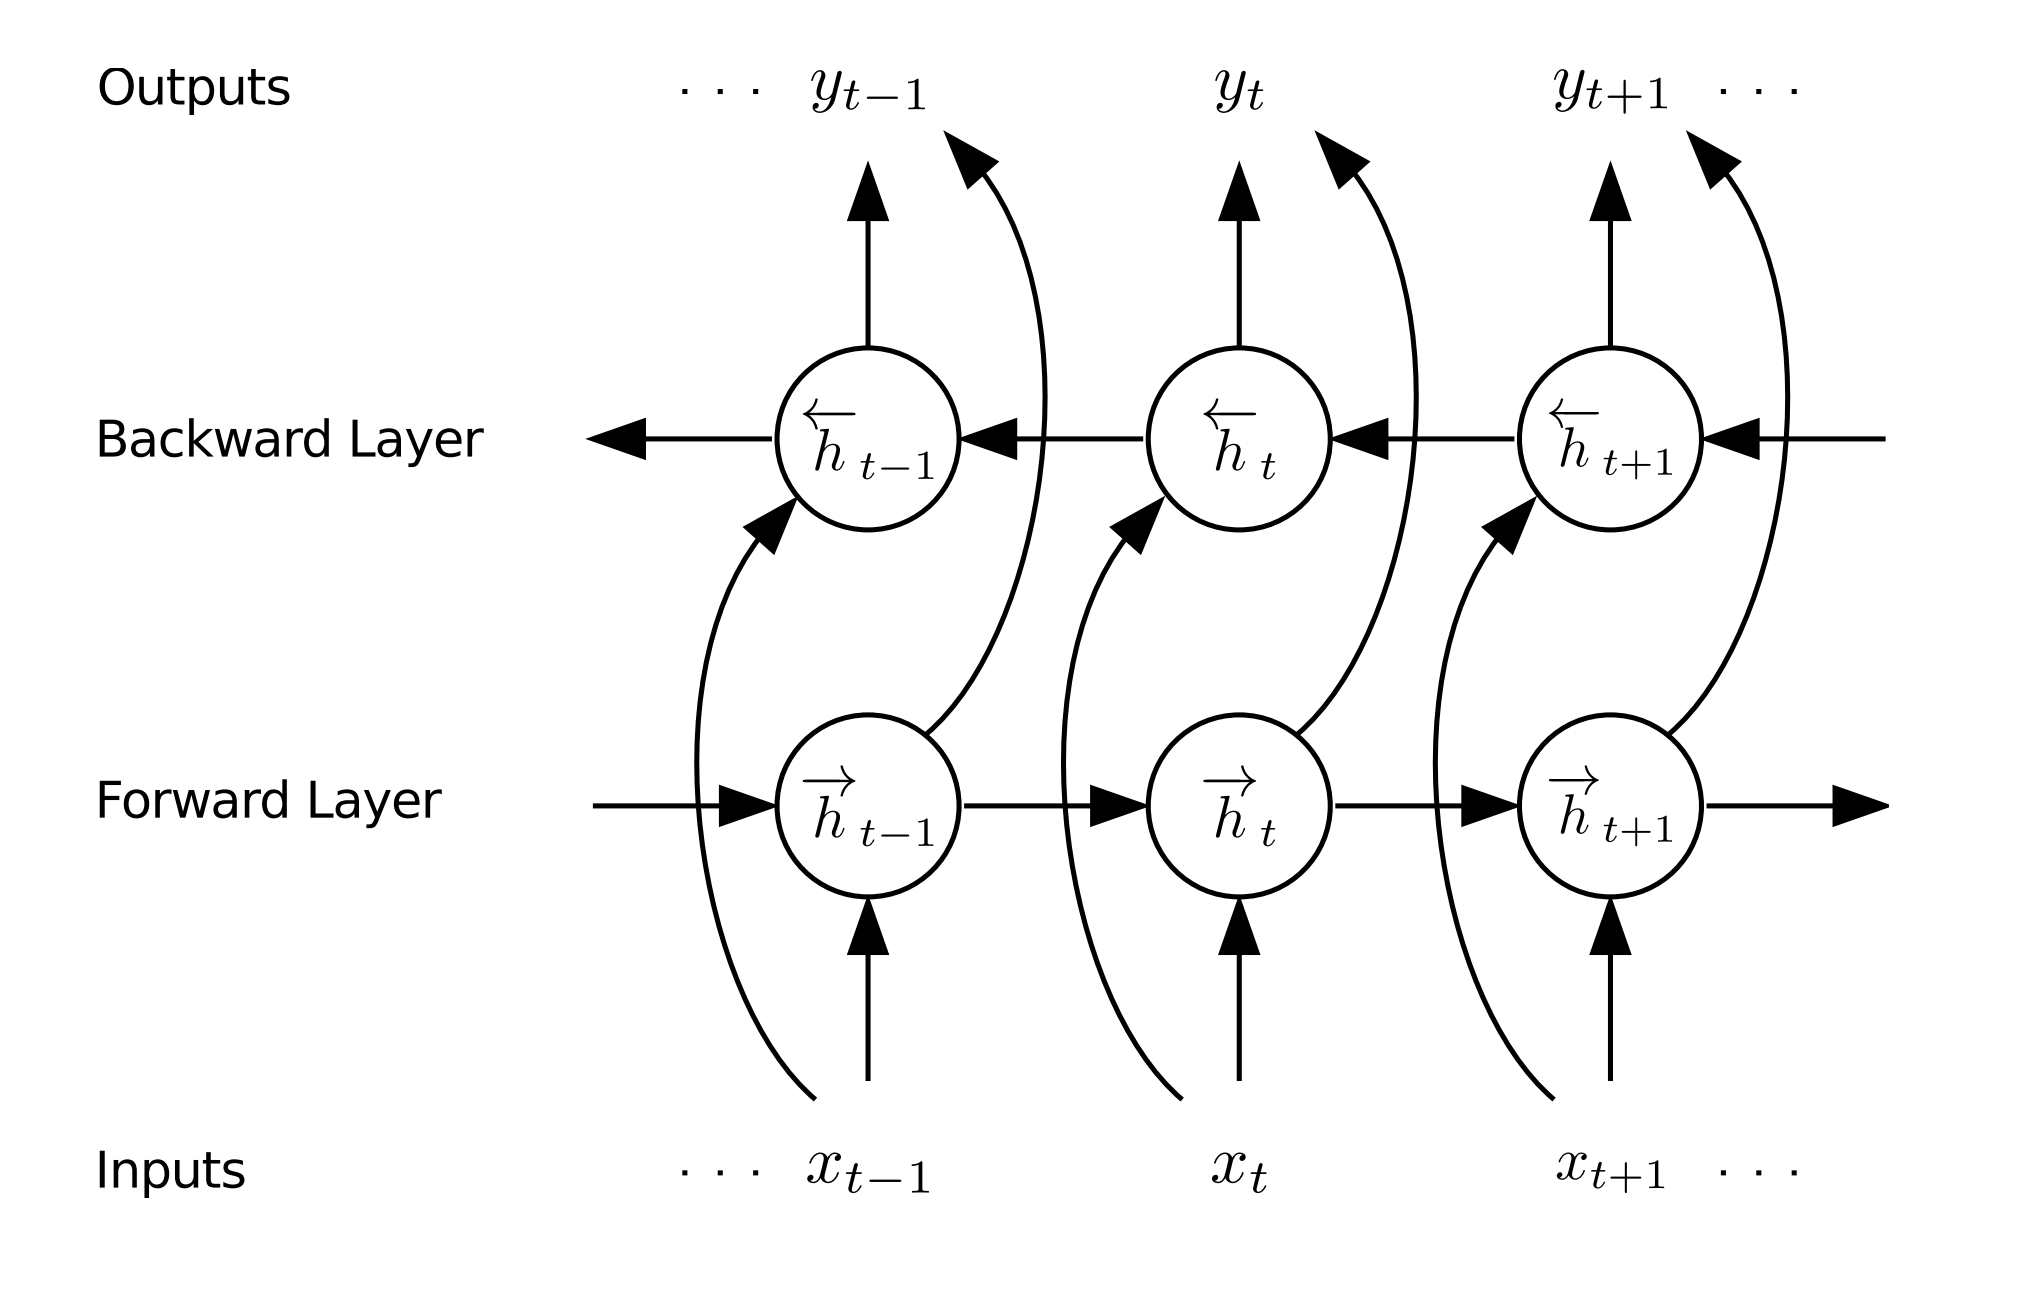
\includegraphics[width=10cm]{Bi-LSTM} \\
  \caption{Bi-directional LSTM \cite{graves2013speech}.}
  \label{fig:bi-lstm}
\end{figure}
In a sequence prediction task, in which one has access to both past and future input features for a given point in time, a bidirectional LSTM network as depicted in \ref{fig:bi-lstm} can be applied as proposed by Graves et al. \cite{graves2013speech}. In this way, it is possible to make us of past features via the forward state and future features via the backward states. Forward and backward passes are executes similarly to 



The forward and backward passes over the unfolded network over time are carried out in a similar way to regular network forward and backward passes, except that we need to unfold the hidden states for all time steps. We also need a special treatment at the beginning and the end of the data points. In our implementation, we do forward and backward for whole sentences and we only need to reset the hidden states to 0 at the begging of each sentence. 




\section{Anomaly Detection \label{sec:anomaly-detection}}
\textit{Anomaly detection} describes the general problem of finding subsets or patterns in data, that do not conform to a defined notion. These patterns are often referred to as outliers or anomalies.

Anomalies can arise in datasets for various reasons, like system errors, fraud or malicious activities. It often might appear to be straight-forward to define normal regions, and declare all data laying outside of these regions as anomalies. Unfortunately, finding these normal regions is in fact very difficult, since it might not always be possible to capture the nature of \textit{normal} data in its completeness, due to lacking data or the unsharp border of normal and abnormal. Consider figure \ref{fig:anomaly_dataset}, which illustrates the presence of normal regions and anomalies in a dataset. The datapoints in the regions $D_1$ and $D_2$ are considered normal, since the majority of observations lie in these regions. Points that are sufficiently far away, like the points in regions $A_1$ and $A_2$ are considered anomalies. But consider also the points $B_1$. Should they be marked as normal or abnormal? Are the borders around $D_1$ and $D_2$ correct, or are they not sufficiently broad, due to the lack of enough normal training examples? 
Additionally to the difficulty of finding correct division of normal and abnormal, normal behaviour can be subject to constant evolution in a dynamic system, thus making previous definitions of \textit{normal} behaviour wrong, obsolete or incomplete. Additionally, it is often hard or impossible to obtain labeled data for the desired domain, thus hindering the training and verification of a model \cite{chandola2009anomaly}.

Due to the difficulties arising from the aforementioned constraints, solutions to the problem of anomaly detection are usually very domain-specific, influenced by the form in which data is available, labeled or unlabeled and the form of anomalies which are to be detected. Solutions presented by researchers feature techniques from various fields, including data mining, statistics, machine learning which are applied to the domain in question \cite{chandola2009anomaly}. Figure \ref{fig:anomaly_technique} outlines the central steps involved in finding an appropriate anomaly detection technique to a given problem.


\begin{figure}[h]
  \centering
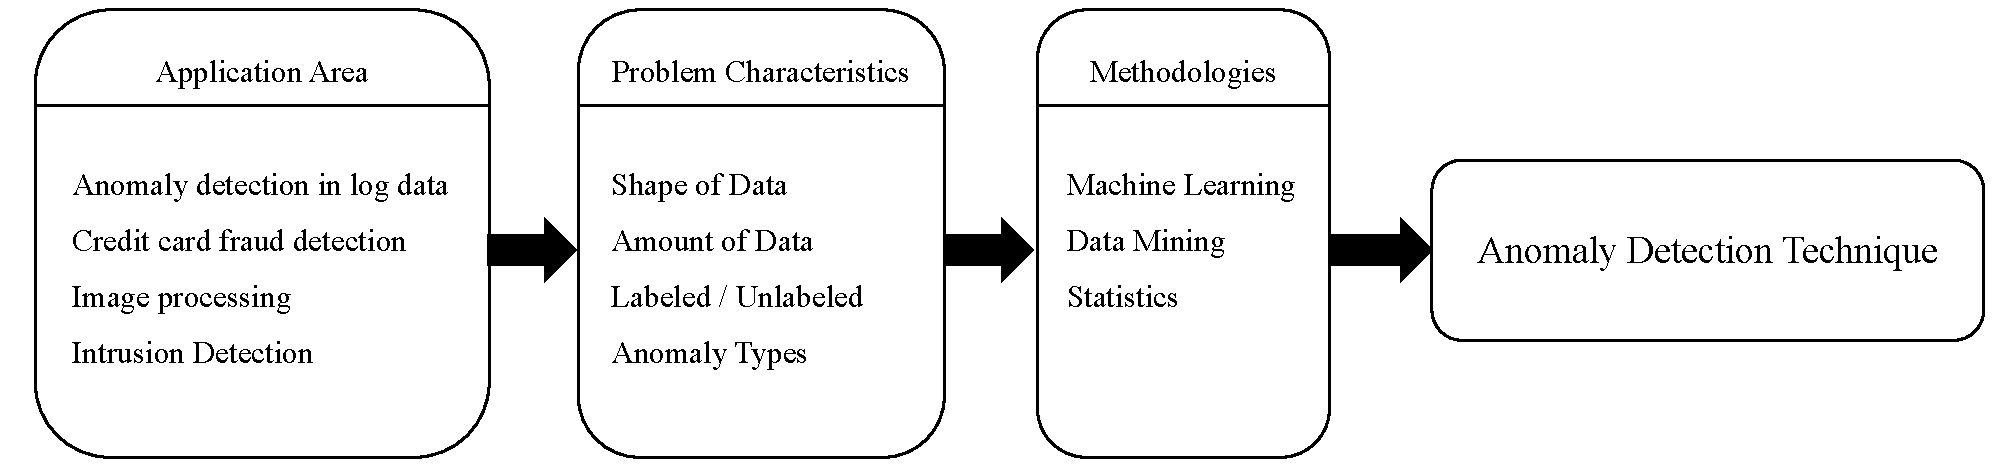
\includegraphics[width=15cm,height=3.5cm]{anomaly_detection_techniques.pdf}\\ 
  \caption{Schema of the development of an anomaly Detection technique \cite{chandola2009anomaly}.}
  \label{fig:anomaly_technique}
\end{figure}

\begin{figure}[h]
  \centering
  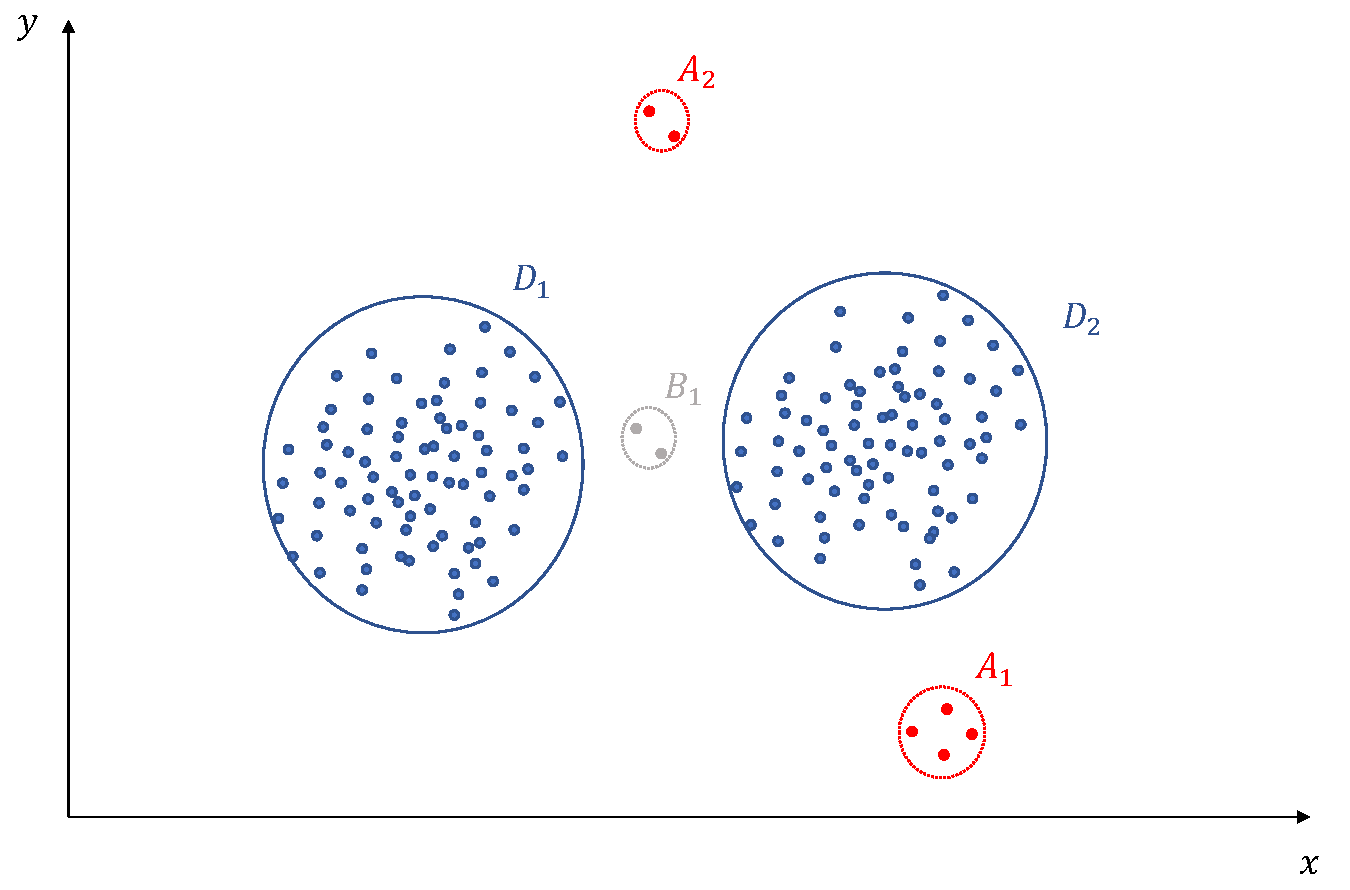
\includegraphics[width=15cm]{anomalies.pdf}\\
  \caption{Example of anomalies in a dataset.}
  \label{fig:anomaly_dataset}
\end{figure}


\section{Natural Language Processing \label{sec:natural-language-processing}}

Natural language processing (NLP) involves the engineering of computational models to solve practical problems in understanding human languages. Having initially relied on processing involving statistics, probability and machine learning, the recent boost in available computational power with GPUs, allowed deep learning to raise the bar for many NLP-tasks. NLP can be broadly divided into two categories, namely \textit{base concepts} which deal with the fundamentals of understanding language, and concrete applications by means of these very concepts, although the border between the two is often fluent. Base concepts include \textit{language modelling}, \textit{morphological processing} (find segments within words), \textit{syntactic processing} (how different words and phrases relate to each other within a sentence) and \textit{semantic processing} (understanding the meaning of words), whereas applications include areas such as text translation, classification of documents, summarisation of texts, extraction of information and many more.
\subsection{Word embeddings}
Language modelling can be viewed as an essential piece of probably any practical application of NLP. Generally speaking, it involves creating a model to predict words given previous words by finding appropriate representations for words through analysing the relations of words within their context. Numeric vectors, which represent single words, obtained by language model techniques are called \textit{word embeddings} \cite{otter2020survey}. For example, the word "Olympics" appears often in the context or close to words like "athlete", "running" or "tournament" but rather rarely next to words like "microphysics" or "chicken". These relationships can be translated into a vector that describes how the word "Olympics" is used within a language \cite{mittechnologyreviewkingqueen}. Word embeddings can be retreived either by Principle Component Analysis or by using deep neural network models and capturing their internal states.
\subsection{Bert \label{Bert}}
The functionality of a language representation model will be outlined on the basis of Bert (\textbf{B}idirectional \textbf{E}ncoder \textbf{R}epresentations from \textbf{T}ransformers) by Devlin et al. \cite{devlin2018bert}. The model architecture is a multi-layer bidirectional Transformer encoder. The encoder maps an input sequence of symbol representations to a sequence of continuous representations. The transformer architecture introduces self-attention and fully connected layers on top of the encoder structure, which has been shown to be superior in quality and is significantly cheaper to train \cite{vaswani2017attention}.

Training includes two steps: \textit{pre-training} and \textit{fine-tuning}. Pre-training involves training on unlabelled data over various pre-training tasks. Finetuning then uses the weights initialised with the parameters obtained from pre-training, re-calibrating them using labelled data.

For pre-training, they extract sentences from a large unlabelled corpus like English Wikipedia. The obtained sentences are then transformed into tokens, and separated by pre-defined separation symbols, \verb![CLS]! for the beginning of a sentence, \verb![SEP]! for the ending of sentences as illustrated in figure \ref{fig:bert}. They then proceed with the first task, namely Masked Language Model (MLM). For this purpose, they mask 15\% of words with the special \verb![MASK]! token, and then predict these tokens. The second task is Next Sentence Prediction (NSP), where sentences \verb!A! and \verb!B! are separated with the aforementioned \verb![SEP]! token, as it can be again seen in figure \ref{fig:bert} are marked with the label \verb!isNext! if \verb!B! follows \verb!A! or \verb!notNext! if the following sentence is a random sentence, with both cases occurring 50\% of the time. After the computationally expensive pre-training is done, taking 4 days of training on 16 cloud TPUs for one language \cite{googlebert}, fine-tuning can be done on any downstream NLP task in at most one hour on one cloud TPU, for example the Stanford Question Answering Dataset (SQuAD v1.1) by Rajpurkar et al. \cite{rajpurkar2016squad}, a collection of 100k crowd-sourced question/answer pairs, or the General Language Understanding Evaluation (GLUE) benchmark by Wang et al. \cite{wang2018glue}, which involves various natural language understanding tasks. 


\begin{figure}[h]
  \centering
  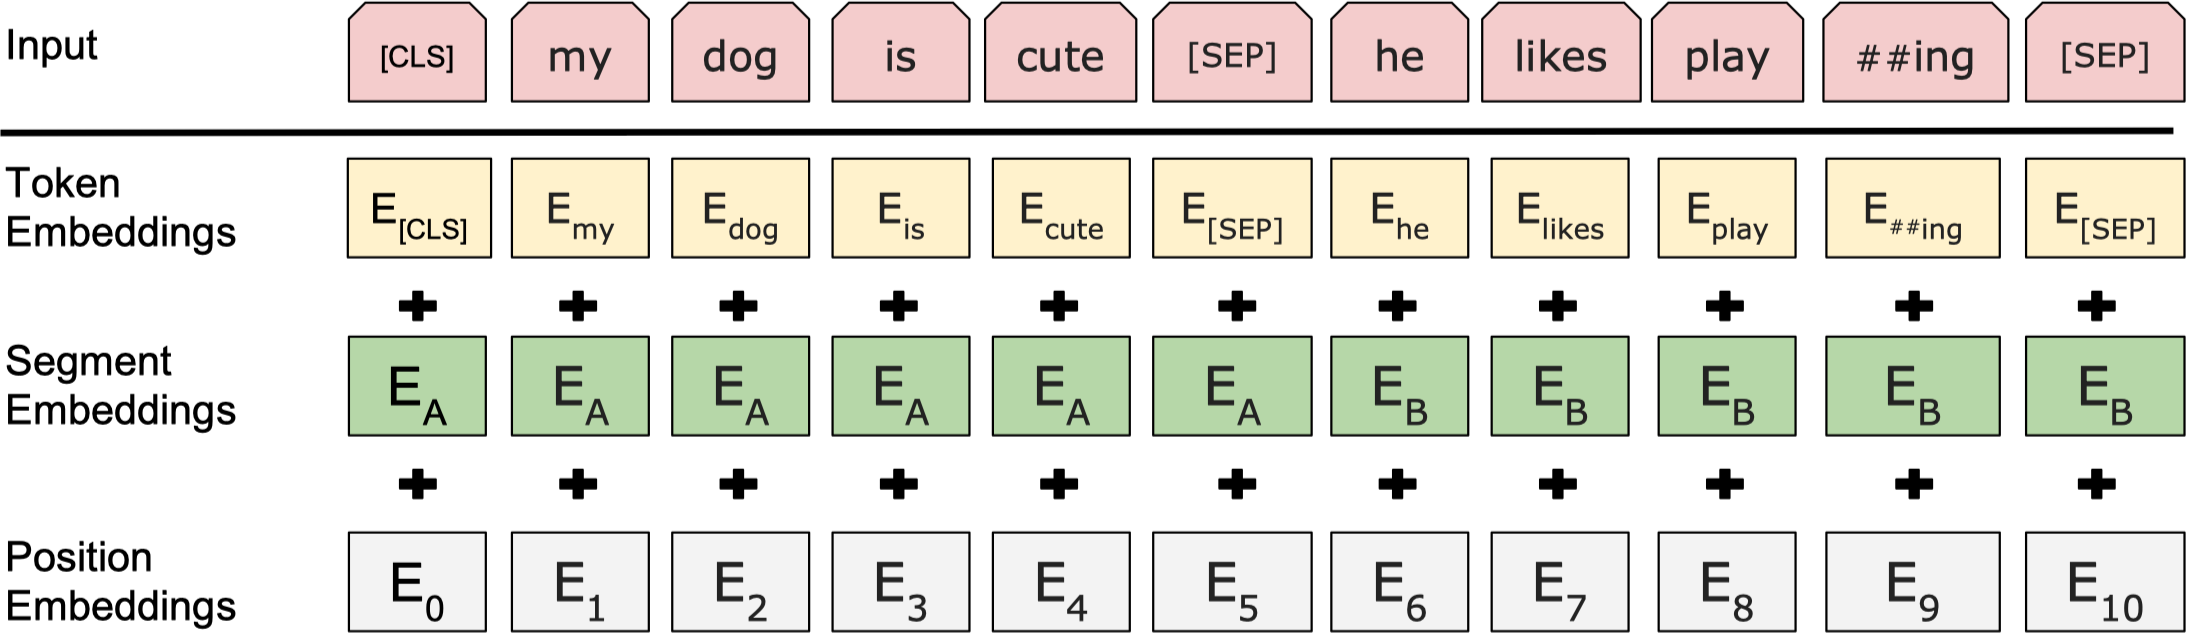
\includegraphics[width=15cm]{bert2.png}\\
  \caption{Bert}
  \label{fig:bert}
\end{figure}


\begin{comment}
\begin{figure}[h]
  \centering
  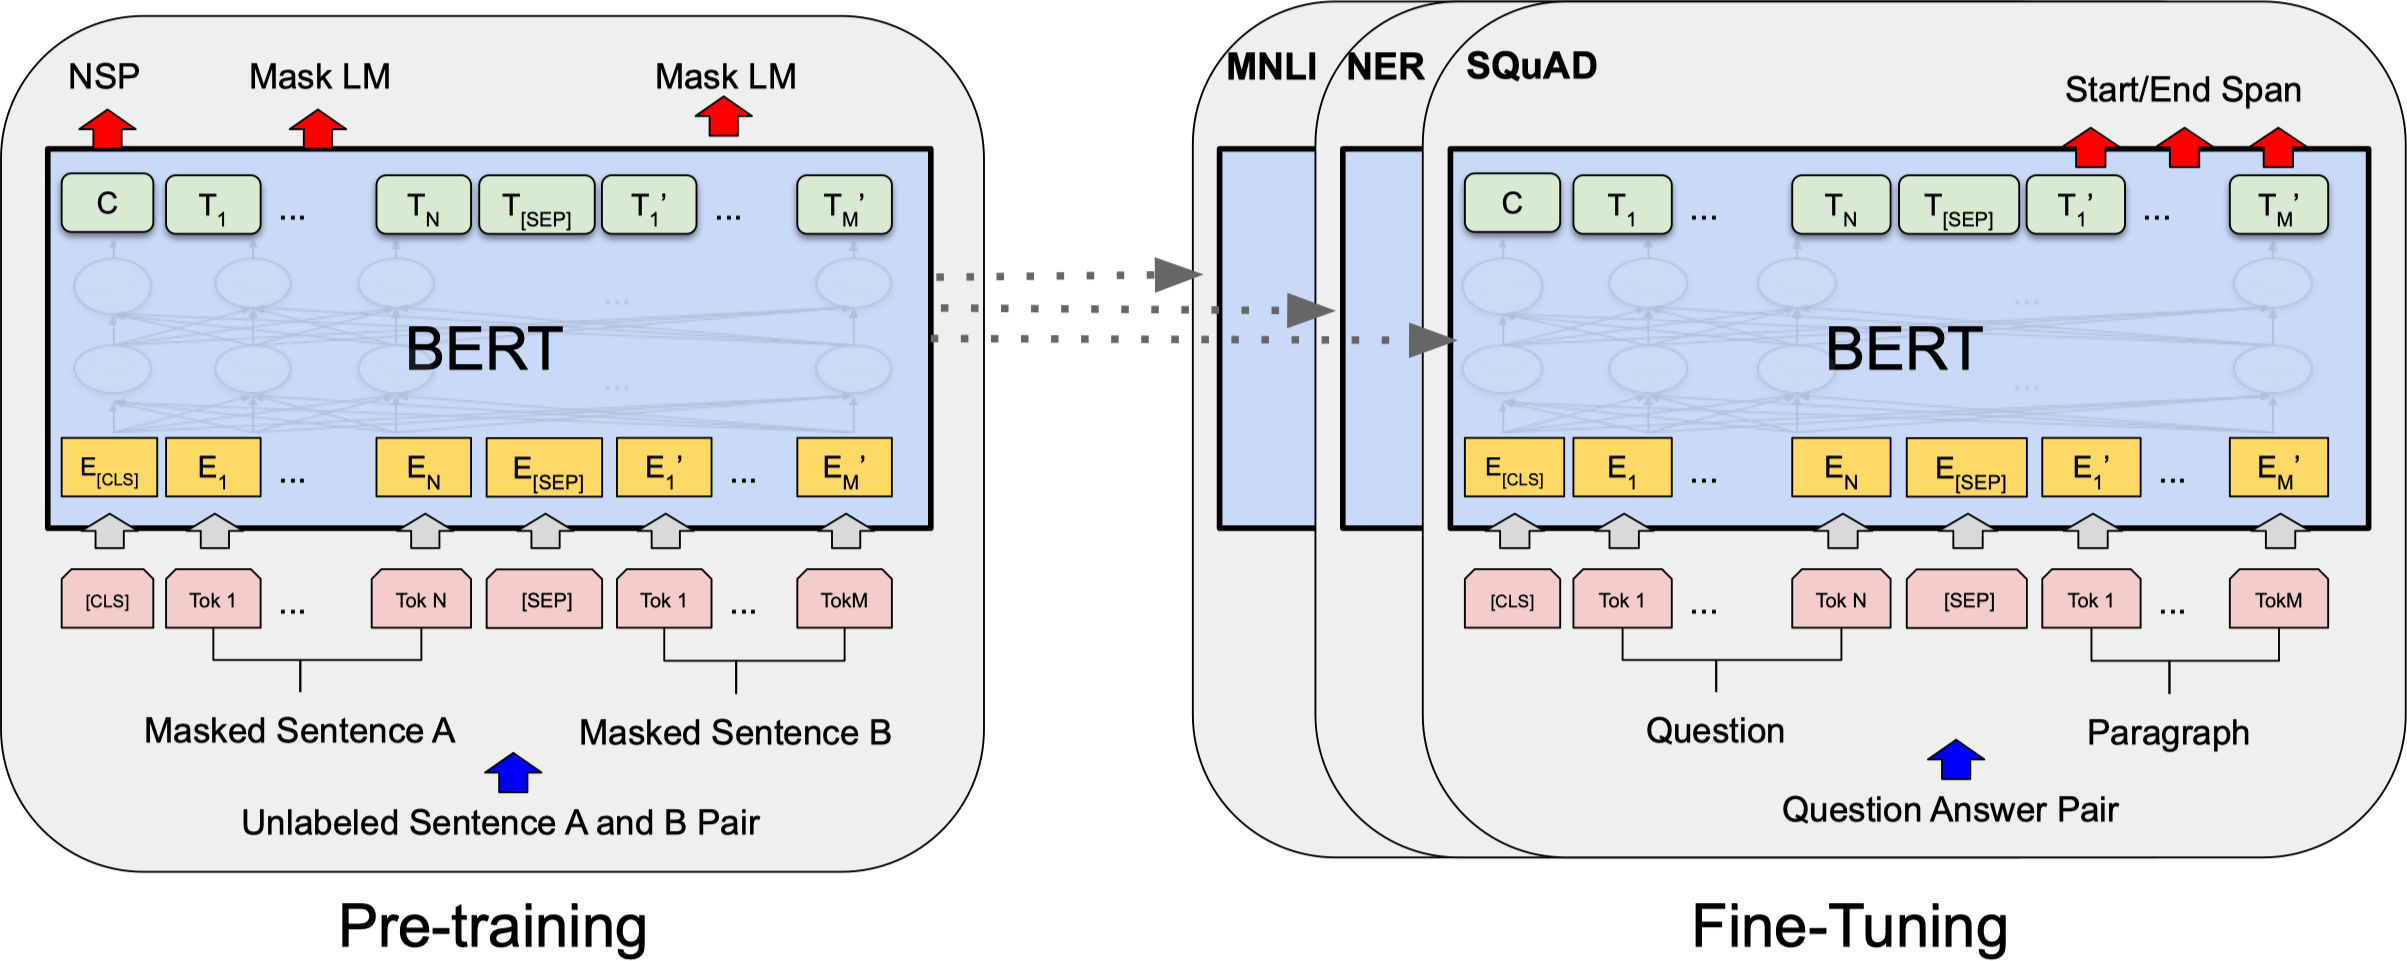
\includegraphics[width=15cm]{bert.png}\\
  \caption{Bert}
  \label{fig:bert}
\end{figure}
\end{comment}

\begin{comment}
Generally, there are two main categories of log sequence anomalies: sequential and quantitative anomalies \cite{meng2019loganomaly}. Programs are usually executed according to static sequences, and the order of the respective log statements that are being produced, is a result of these executions. A sequential anomaly occurred, when a given sequence departs from a pattern that has been defined as normal. Works in this area include DeepLog \cite{du2017deeplog}.
Additionally, program executions have constant linear relationships - these can be captured by the quantitative relationships of logs. If these relationships are not met under all circumstances, an anomaly has occurred. Existing works in the area include PCA based approaches over log message counter \cite{xu2010robust} \cite{xu2009detecting} and LogClustering \cite{lin2016log}, but there are also deep learning based approaches to learn sequences of logs, like DeepLog \cite{du2017deeplog}. The main limitation of these approaches is that they use log event template indices as input to predict sequences. 

To overcome the shortcomings of previous approaches, it is worthwhile to consider recent developments in natural language processing. In order for a machine to process information given in natural language, a suitable representation for the given text has to be found. Learning representations of words has been a dynamic area of research, using neural \cite{blitzer2006domain} \cite{devlin2018bert} \cite{radford2019language} \cite{merity2017regularizing} \cite{yang2017breaking}, statistical \cite{brown1992class} and other machine learning methods \cite{ando2005framework} \cite{pennington2014glove}. Recently, we have seen considerable improvements in both the (multi-) task solving capabilities and efficiency of deep learning approaches. Because of their capabilities of memorising sequential context in language, RNNs \cite{mikolov2010recurrent} have often been the architecture of choice \cite{merity2017regularizing} \cite{yang2017breaking} in the past years. Decidedly designed cells to memorise such context make them computationally expensive, making it difficult to scale to large corpora \cite{wang2019language}. The transformer architecture introduces self-attention and fully connected layers, which has been shown to be superior in quality and is significantly cheaper to train \cite{vaswani2017attention}. BERT \cite{devlin2018bert} and GPT-2 \cite{radford2019language} provide state of the art results in various NLP tasks. There exist a variety of practical applications, such as information retrieval \cite{manning2008introduction}, question answering \cite{tellex2003quantitative}, paraphrasing \cite{dolan2005automatically}, natural language inference \cite{bowman2015large}, document classification \cite{sebastiani2002machine}. They are trained in an unsupervised manner on publicly available datasets like Wikipedia, or millions of web pages accumulated in one dataset, to obtain a more diverse dataset \cite{radford2019language}. This allows them to achieve state of the art results in various language modeling tasks like question answering \cite{reddy2019coqa} or language inference without specific modifications of the model to solve a certain task \cite{devlin2018bert}, making them much more universally applicable than older approaches like word2vec \cite{mikolov2013distributed} or GloVe \cite{pennington2014glove}. There are recent studies \cite{zhang2019robust} \cite{meng2019loganomaly} which utilise such pre-trained word embeddings to provide a more meaningful representation of log events, being able to take into account their semantics. 
In this section, the necessity for anomaly detection with log events represented by word embeddings is further elaborated. For this purpose, the necessary methods like log parsing, 
Log messages are the result of the insertion of a variable part in a logging instruction (e.g. \textit{printf("Instance \%s shut down with errors, \%s)} in software code that is being output during execution. The constant parts can usually be found in source codes written by developers, while the variable parts are inserted dynamically during execution. As these logs are unstructured text, have to undergo certain pre-processing steps before they can be analysed for anomalies. Each log event can be parsed into a log template, leaving only the constant part, as it can be seen in figure \ref{fig:parsing}.
\end{comment}


\section{Log Parsing \label{sec:backgroundlogparsing}}
Due to the unstructured nature of log data, the first crucial step in anomaly detection on log data is parsing. Raw log messages consist of a constant and a variable part, with the constant part remaining identical for every occurrence, while the variable part records runtime information and varies among different event occurrences. The goal of log parsing is to separate the \textit{constant} and \textit{variable} part of a raw log message \cite{he2017towards}\cite{zhu2019tools}. Figure \ref{fig:parsing} shows how logging statements from Java source code are parsed. The logging statements variable parts \verb!block!, \verb!block.getNumBytes()! and \verb!inAddr! are dynamically interpreted at runtime and replaced by their respective values. The resulting log message is then printed with additional customisable values (timestamp, logging level and component) by the respective logging framework. The structured log is then produced by the log parser, separating the constant part, which is also called a \textit{template} (\verb!Received block <*> of size <*> from /<*>!) from the variable parts (\verb!blk_-562725280853087685, 67108864! and \verb!10.251.91.84!), replacing the variable parts inside the constant parts with a pre-defined token - "\verb!<*>!" in this example.

Log parsing is usually the first step in order to perform a log analysis task. Log parsing enables enables searching, filtering, grouping and mining of logs. Applications include usage analysis at Twitter \cite{lee2012unified} or workload modelling \cite{barham2004using}. Logs can also be used as data sources for performance modelling \cite{chow2014mystery} where performance improvements of a system can be validated using log data. A very prominent application of log parsing is anomaly detection. Since logs record execution information of a system, they are a valuable data source for identifying abnormal behaviour of a system \cite{zhu2019tools}.

There exist offline and online log parsers, offline meaning that it first reads and analyses the whole dataset first before applying the parsing model, while online parsers adjusts the parsing model gradually during the parsing process \cite{he2017drain}. Log parsers employ various concepts and techniques in order to parse logs - a few of them are summarised here:
\begin{itemize}
\setlength\itemsep{0em}
	\item \textit{Frequent Pattern Mining} involves finding sets of patterns, in this case templates, that appear frequently in a data set. The procedure can be outline as follows: Iterating over the log data several times, while building frequent sets of tokens, followed by grouping log messages in clusters, and then extracting event templates from each of the clusters.
	\item Log parsing can be viewed as a \textit{clustering} problem. All approaches can be roughly outlined as clustering templates hierarchically based on a defined metric, for example the weighted edit distance between pairwise log messages \cite{zhu2019tools}.
	\item Some proposed methods utilise special heuristics, 	exploiting the unique characteristics of log messages. IPLoM first identifies frequent words occurring more frequently than a threshold value, then extracts combinations of these words that occur in each line in the data set, marking them as cluster candidates, and finally selecting the candidates the occur more often than a threshold value as clusters \cite{makanju2009clustering}. Drain employs a parse tree with fixed depth. It first preprocesses the incoming messages with regular expressions based on domain knowledge, then search a log group for that message, with log groups being leaf nodes. If a suitable group is found, it matches the message to that group, if not, then a new group is created \cite{he2017drain}.
\end{itemize}


\begin{figure}[h]
  \centering
  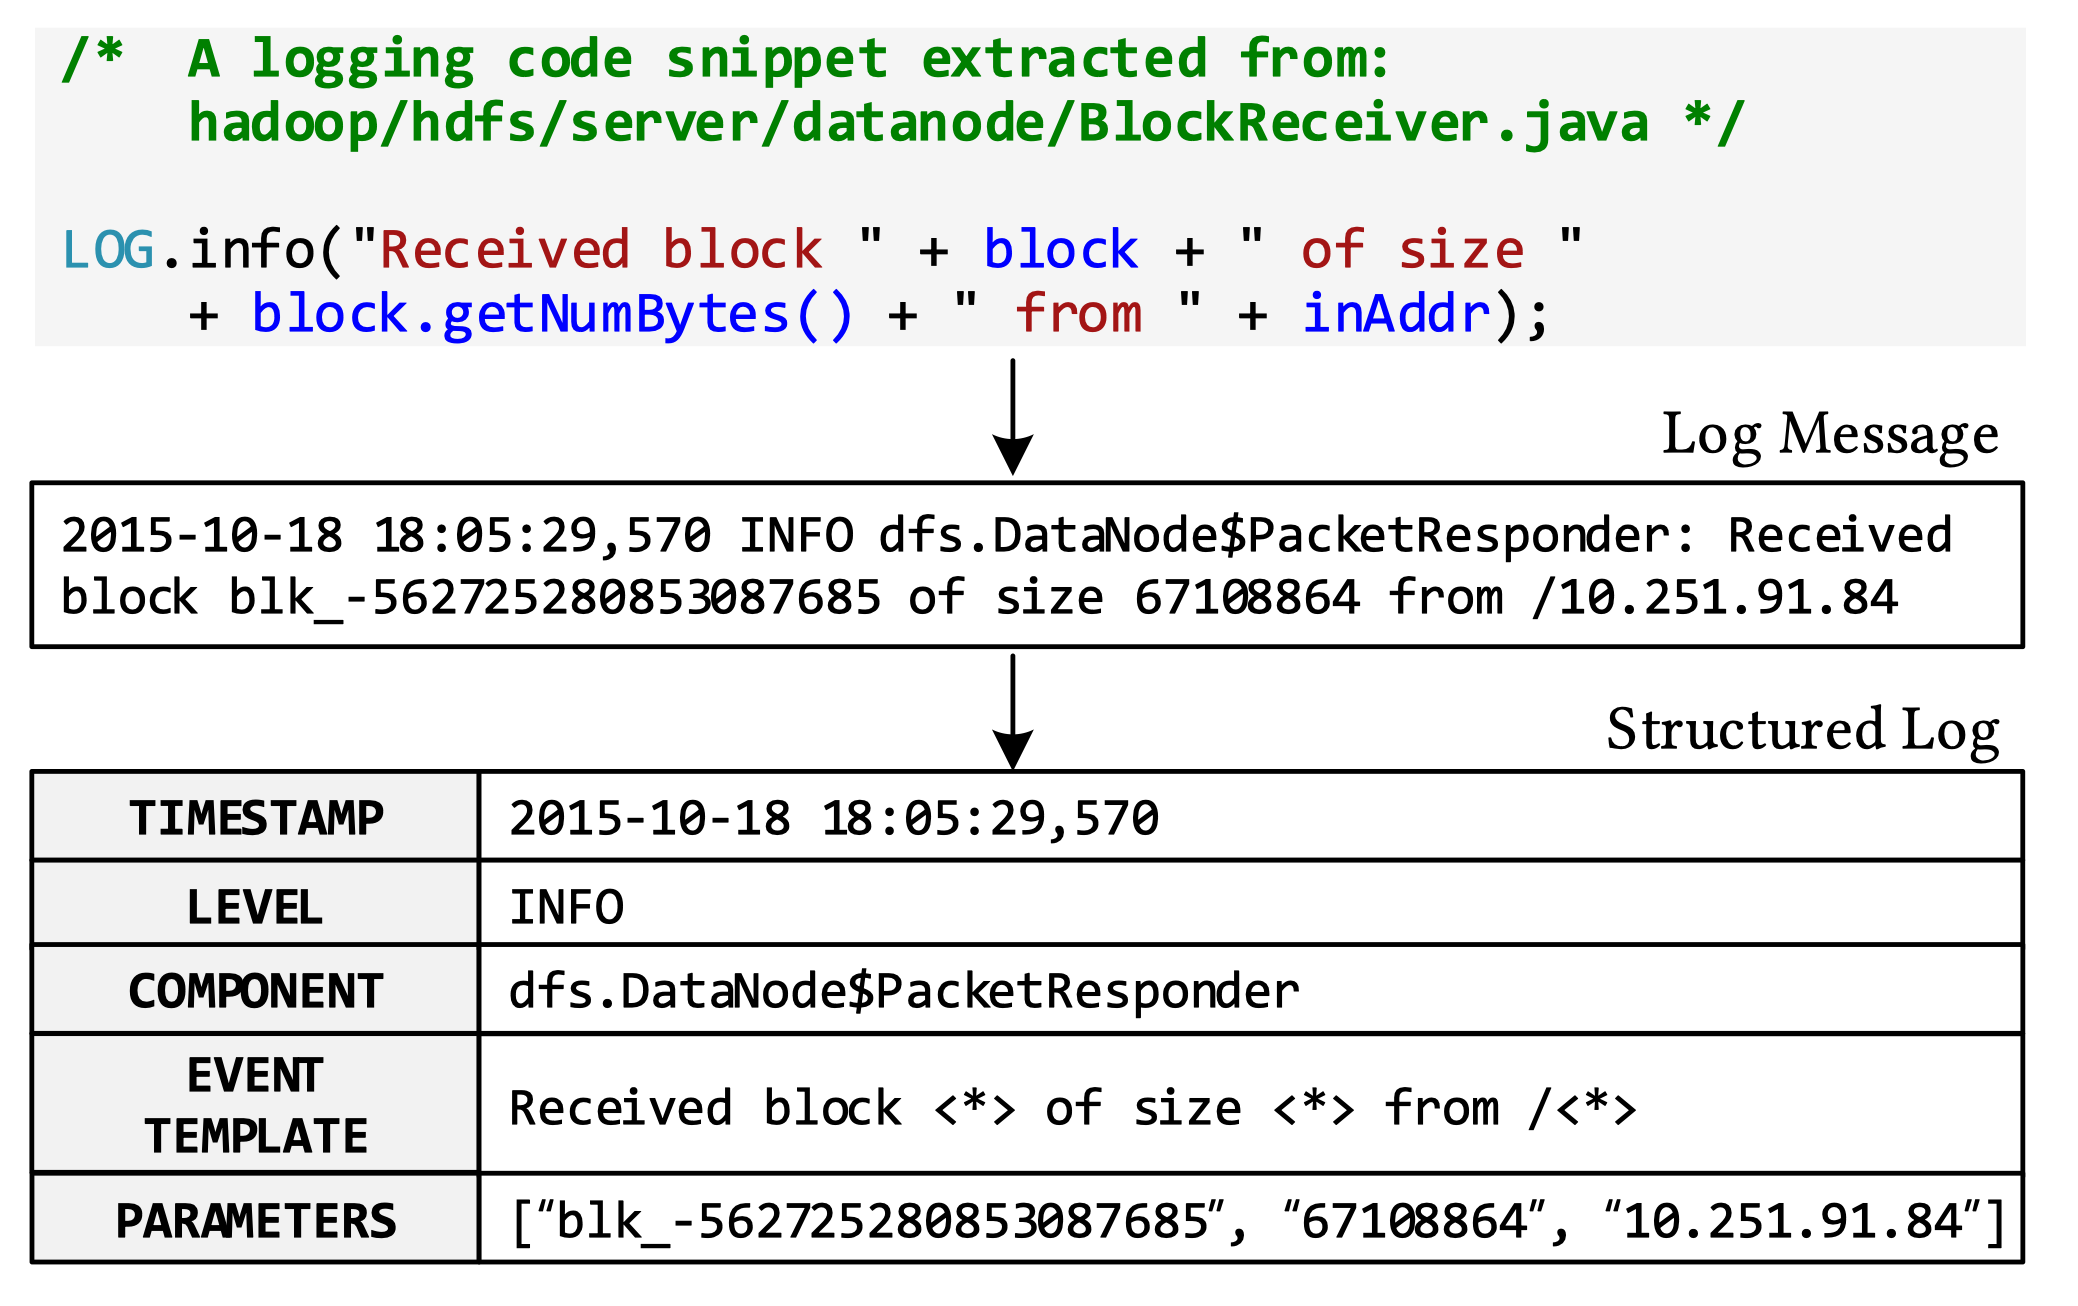
\includegraphics[width=12cm]{log_parsing.png}\\
  \caption{Schematic execution of log parsing \cite{zhu2019tools}}
  \label{fig:parsing}
\end{figure}

